\section{Development:}

After starting the etching process to make our circuit board we need to cut the copper plate at the size of the {\itshape layout}. In our case we needed of {\itshape 10mm} of height per {\itshape  6mm} of width approximately. So, using the cutter we {\itshape mark} the copper plate several times like in Figure 3.0 until the copper plate split easily ( Figure 3.1 ). The we can start the etching process. \hfill \break

\begin{figure}[H]
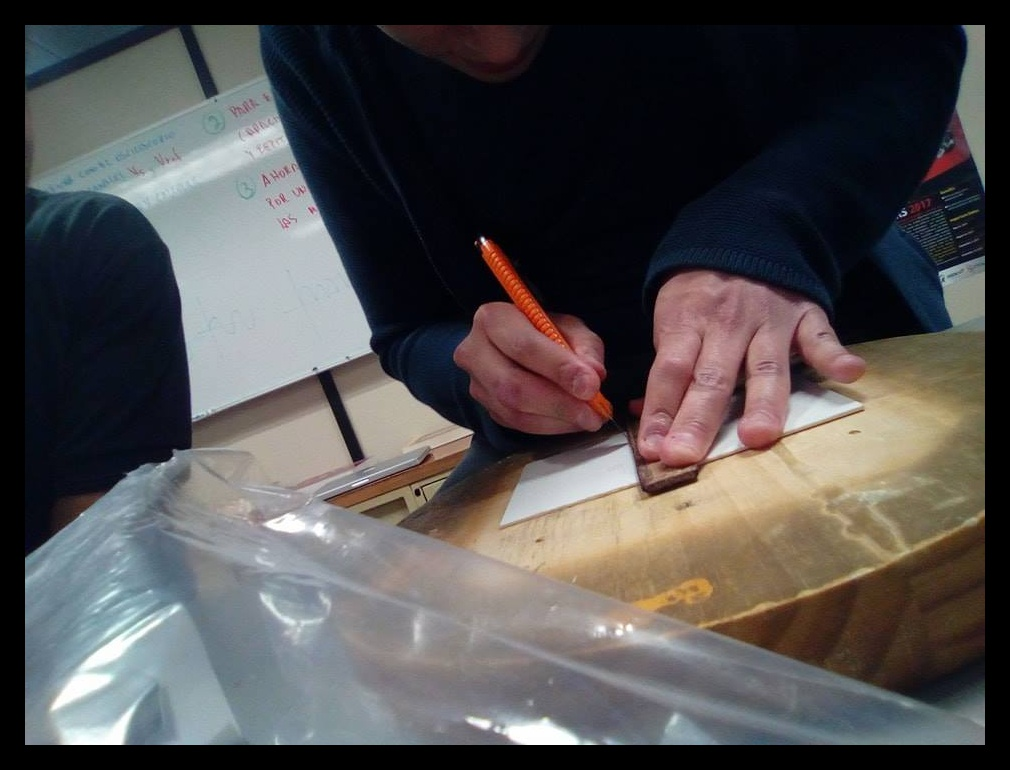
\includegraphics[height = 7cm, width = 16.5cm]{1a.jpg}
\centering \linebreak \linebreak {\small Figure 3.0: Cutting the cooper plate.}
\end{figure} \hfill \break

\begin{figure}[H]
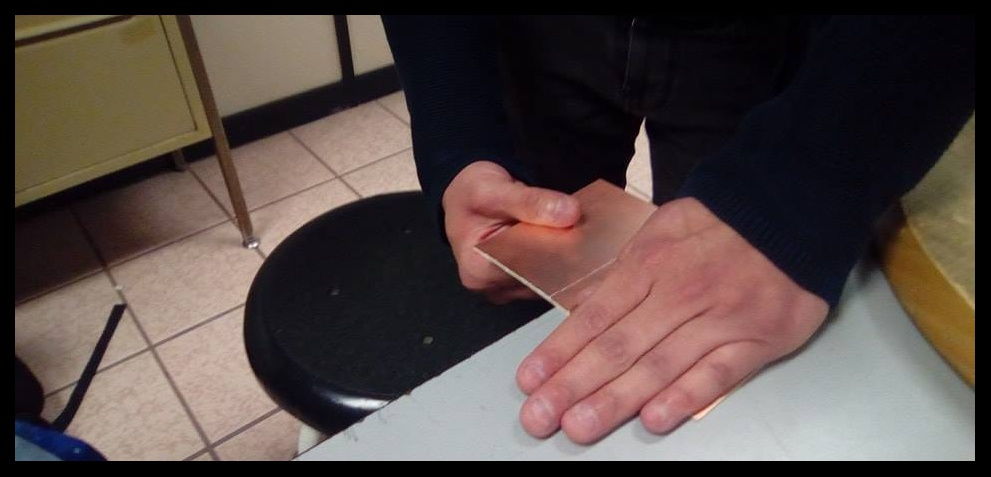
\includegraphics[height = 7cm, width = 16.5cm]{1b.jpg}
\centering \linebreak \linebreak {\small Figure 3.1: Splitting the cooper plate.}
\end{figure}

\pagebreak